\section{Results}

\subsection{Proof of concept}

The oil-treated nitrocellulose membrane was found to provide a uniform background relatively free of artifact for the purposes of imaging. The grey-level distributions of ten samples of \lq background' were plotted (Fig.~\ref{fig:BackgroundDist}) and found to approximate a scaled Gaussian distribution:

\begin{equation}
	\frac{a}{\sqrt{2 \pi \sigma^2}} \exp \left( \frac{-(x-\bar{x})^2}{2 \sigma^2} \right)
\end{equation}

\noindent where $a$ is a scaling factor, $\bar{x}=164$ and $\sigma=4$. This narrow distribution represents a relatively uniform image background, which is essential for accurate grey-level thresholding, whereby the object and background are partitioned based on an analysis of a bi-modal histogram (see Fig.~3.6).

\begin{figure}[htbp]
	\centering
	\pstool[width=10.5cm]{../C3/BackgroundDist}{
		\psfrag{N}[Bc]{\al Number of Pixels}
		\psfrag{L}[Bc]{\al\hspace{2mm}Luminance}}
	\caption{Distribution of grey-level luminance values (\emph{in grey}) for 10 background samples ($320 \times 240$ pixels). The histograms approximate a Gaussian distribution (\emph{black dashes}) with $\bar{x} = 164$ and $\sigma = 4$.}
	\label{fig:BackgroundDist}
\end{figure}

The rudimentary assay was used to identify key developments in the growth of \emph{A. oryzae} on a solid substrate. Spore germination was first noted at 8 hours but was not widespread until 9~hours post-inoculation (Fig.~\ref{fig:KeyPointa}); germ tubes emerging from a cluster of spores appear to radiate away from the cluster's centre of mass (Fig.~\ref{fig:KeyPointb}). The beginnings of hyphal branching were first noted at 16~hours when small nodules began to form on the primary hyphae (Fig.~\ref{fig:KeyPointc}). The emergence of a second germ tube from the spore was often observed at this time (Fig.~\ref{fig:KeyPointd}).

\begin{figure}[tb]
	\centering
	\subfloat[]{\label{fig:KeyPointa}\fbox{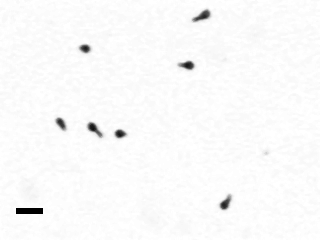
\includegraphics[width=5cm]{../C3/SporeGermination7h}}}
	\hspace{0.5cm}
	\subfloat[]{\label{fig:KeyPointb}\fbox{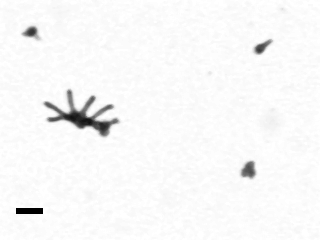
\includegraphics[width=5cm]{../C3/SporeCluster8h}}}
	\\
	\subfloat[]{\label{fig:KeyPointc}\fbox{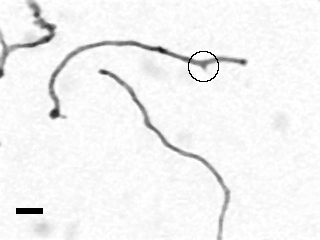
\includegraphics[width=5cm]{../C3/Branching16h}}}
	\hspace{0.5cm}
	\subfloat[]{\label{fig:KeyPointd}\fbox{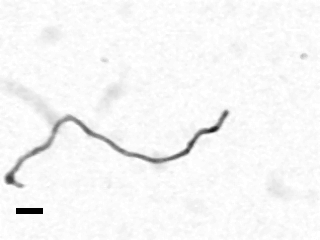
\includegraphics[width=5cm]{../C3/2ndGermTube16h}}}
	\caption{(a) Germ tube emergence from individual spores at 9~h (b) Germ tube emergence from spore cluster; the germ tubes appear to radiate outward away from the centre of mass (c) Emergence of branching hypha at 16~h (d) Emergence of 2nd germ tube at 16~h. All images captured at $\times 400$ magnification (Bars: \mic{15}).}
	\label{fig:KeyPoints}
\end{figure}

The application of immersion oil permitted the use of oil immersion lenses directly on the sample, thereby allowing high-power magnification and the imaging of fine details (Fig.~\ref{fig:HighMags}). While useful for the identification of septae, the imaging of hyphae at high magnification may also be of interest as a means of tracking hyphal morphogenesis \cite{dieguez-uribeondo2004}, thus potentially providing kinetic data on the evolution of apical and sub-apical regions over time. Such analyses may be of value in studying the response of hyphae to changes in environmental conditions and/or metabolic activity. It has previously been demonstrated, for example, that the shape of the apical compartment of certain \emph{Aspergilli} varies with the specific growth rate \cite{muller2000}, while Haack and colleagues reported an increase in hyphal tip size during the feeding phase of fed-batch culturing of \emph{A. oryzae} \cite{haack2006}. Further studies have found that the hyphal diameter of \emph{A. oryzae} is significantly reduced when the organism is starved of glucose \cite{pollack2008}. However, such investigations were beyond the scope of this study.

\begin{figure}[htbp]
	\centering
	\subfloat[]{\label{fig:GermHighMag}\fbox{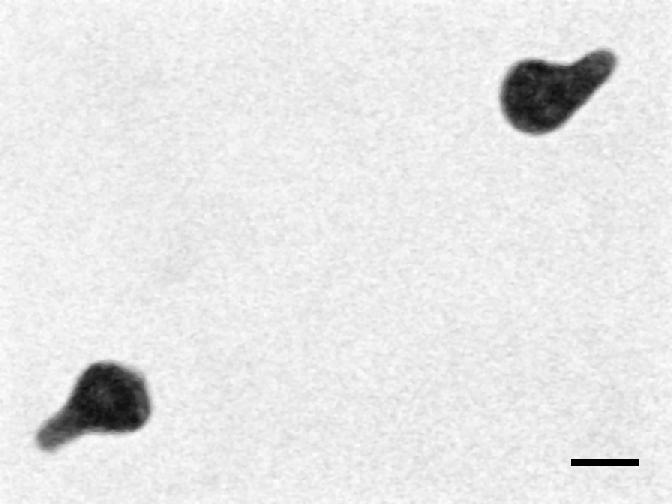
\includegraphics[width=6.5cm]{../C3/GerminationHighMag}}}
	\hspace{0.5cm}
	\subfloat[]{\label{fig:SeptaHighMag}\fbox{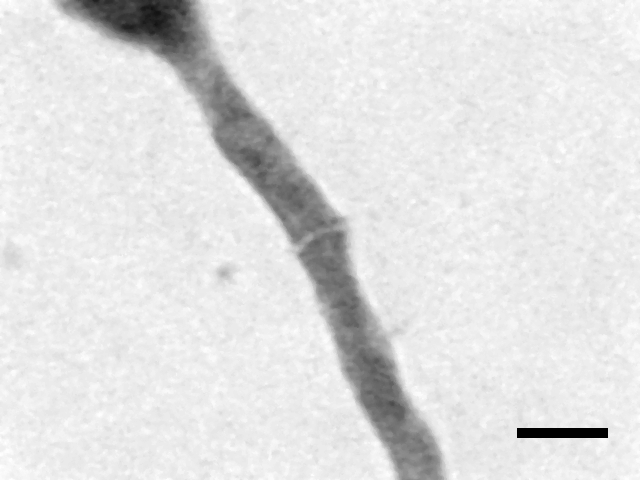
\includegraphics[width=6.5cm]{../C3/Septa1}}}
	\caption{(a) Germ tube emergence and (b) septation in \emph{A. oryzae} visualized on nitrocellulose; the undulating nature of the hyphal surface is also apparent. Images were captured at $\times 1,000$ (Bars: \mic{5}).}
	\label{fig:HighMags}
\end{figure}

\subsection{Assay optimisation}

Further development of the assay was undertaken in an attempt to maximise both the resultant image quality and the speed of assay execution, without compromising cell integrity or disrupting morphological conformations. Investigations focussed on minimising sample drying time and evaluating the effects of this accelerated drying on cell structure.

Contiguous staining of hyphal elements is essential to avoid misinterpretation of the field of view by the image-analysis routines. Staining of membranes while still wet was found to result in non-uniform, patchy staining of hyphae (Fig.\ref{fig:WetDryStain}). While this did not pose significant problems for manual, qualitative examinations, it did result in an over-estimation of the number of discrete hyphal elements within a given sample and, consequently, an underestimation of hyphal length and number of tips when subjected to automated analysis. Within a typical experiment, it was found that up to 80\% ($n = 50$) of the hyphal elements were misinterpreted as multiple objects within samples that were stained while wet. Drying of membranes before staining reduced the incidence of this artifact to less than 2\% of cases.

\begin{figure}[tb]
	\centering
	\subfloat[]{\label{fig:WetDrya}\fbox{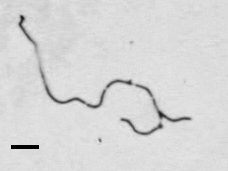
\includegraphics[width=5cm]{../C3/WetStainBW}}}
	\hspace{0.5cm}
	\subfloat[]{\label{fig:WetDryb}\fbox{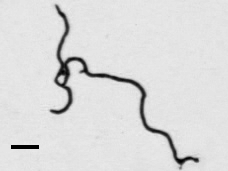
\includegraphics[width=5cm]{../C3/DryStainBW}}}
	\\
	\subfloat[]{\label{fig:WetDryc}\fbox{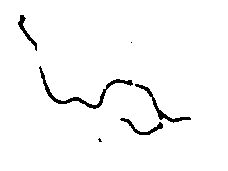
\includegraphics[width=5cm]{../C3/WetStainBin}}}
	\hspace{0.5cm}
	\subfloat[]{\label{fig:WetDryd}\fbox{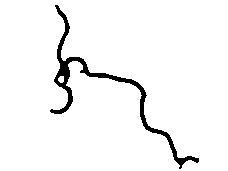
\includegraphics[width=5cm]{../C3/DryStainBin}}}
	\caption{Staining wet membranes resulted in non-uniform stain uptake. (a) Samples of \emph{A. oryzae} on cellulose nitrate membranes were stained while wet immediately upon removal from agar surface; (b) Samples were fixed and then dried at \celc{65} for 75~minutes prior to staining; (c) Binary image resulting from grey-level thresholding of \lq a' (six distinct structures are produced); (d) Binary image of \lq b' (a single hyphal structure produced). Bar: \mic{30}.}
	\label{fig:WetDryStain}
\end{figure}

Within certain limits of time and temperature, the drying of membranes was not found to adversely affect cell morphology. Drying at \celc{25} for 24~hours was without appreciable effect on spore size, but prolonged exposure (up to 72~h) resulted in a reduction of the mean projected area of the spore population (approximately 8\%; Table~\ref{tab:SporeDry}). The drying of samples at temperatures up to \celc{105} had no discernible impact on spore projected area or circularity if performed for a short time (10~min), but caused the cellulose nitrate membrane to wilt. No significant change in spore circularity was observed with any treatment. 

\begin{table}[tb]
	\centering
	\footnotesize
		\begin{threeparttable}
			\caption{Mean projected area ($\Ap$) and mean circularity ($C$) of \emph{A. oryzae} spores subjected to various drying treatments prior to staining, where $n$ is the size of each population. Errors represent 95\% confidence intervals}
			\label{tab:SporeDry}
			\centering
				\begin{tabularx}{(\textwidth - 1cm)}{l X X X r}
					\toprule
					Drying temperature ($^\circ$C) & Drying time (h) & $\Ap$ (\omics) & $C$ & \emph{n} \\ \midrule
					N/A & 0 & 7.7 $\pm$ 0.3 & 0.895 $\pm$ 0.003 & 726\\
					25\tnote{1} & 24 & 8.2 $\pm$ 0.3 & 0.888 $\pm$ 0.003 & 2,915\\
					25 & 72 & 7.1 $\pm$ 0.2 & 0.882 $\pm$ 0.003 & 768\\
					65 & 1.25 & 8.1 $\pm$ 0.1 & 0.887 $\pm$ 0.002 & 2,505\\
					105 & 0.17 & 8.4 $\pm$ 0.1 & 0.886 $\pm$ 0.002 & 2,315\\
					\bottomrule
				\end{tabularx}
			\begin{tablenotes}
				\item [1] Average of two independent experiments.
			\end{tablenotes}
		\end{threeparttable}
\end{table}

An analysis of the size distributions of each population of spores subjected to these treatments provides an additional insight into the impact of accelerated drying (Fig.~\ref{fig:SporeDryDist}). Maintaining the spores at \celc{25} for 24~hours does not result in an appreciable change in the overall shape of the distribution, but extended exposure (72~hours) causes the histogram to narrow significantly, with a considerable reduction in the number of spores recorded at larger projected areas. Drying spores at higher temperatures seems to result in a slight increase in projected area for the population overall. This may be a result of an increase in internal pressure within the spores arising from the increase in temperature, which produces a subsequent increase in volume. However, there is little change in the height or position of the mode of each distribution. A drying treatment of \celc{65} for 1.25~hours was selected for routine use; this enabled acceptable speed of processing without compromising cell morphology or the integrity of the membrane.

\begin{figure}[htbp]
	\centering
	\captionsetup[subfloat]{position=top}
	\subfloat[]{\label{fig:ApsDryT}\pstool[width=10.5cm]{../C3/ApsDryT}{
		\psfrag{F}[Bc]{\al \% Frequency}
		\psfrag{A}[Bc]{\al\hspace{2mm}$\Ap$ (\omics)}}
	}
	\\
	\subfloat[]{\label{fig:ApsDry}\pstool[width=10.5cm]{../C3/ApsDry}{
		\psfrag{F}[Bc]{\al \% Frequency}
		\psfrag{A}[Bc]{\al\hspace{2mm}$\Ap$ (\omics)}}
	}
	\caption{Comparisons of size distributions of populations of \emph{A. oryzae} spores subjected to (a) \celc{25} for 0 ($\bs$), 24 ($\color{gray} \bs$) and 72~hours ($\square$) ($n \approx 700$) and (b) \celc{25} for 24~hours ($\bs$), \celc{65} for 75~minutes ($\color{gray} \bs$) and \celc{105} for 10~minutes ($\square$) ($n \approx 2,000$).}
	\label{fig:SporeDryDist}
\end{figure}

An important caveat to the use of drying procedures was found to be that a fixative be employed to maintain cell structure. Apparent rupturing of hyphal tips was observed in non-fixed samples that were dried prior to staining, with the effect being most pronounced when samples were dried at \celc{65} (Fig.~\ref{fig:BurstTips}). This rendered hyphal elements unsuitable for analysis, because the affected tips were incorrectly classified by the image-analysis system. Typically it was found that approximately 60\% ($n = 70$) of hyphal elements exhibited at least one ruptured tip when dried at \celc{65}, but when samples were fixed before drying, this figure was reduced to approximately 5\% (based on manual observation). Exposure to lacto-phenol cotton blue or fixative caused the membrane to wilt slightly on contact, but extended exposure (up to 30~min) was not found to have any additional impact.

\begin{figure}[tb]
	\centering
	\subfloat[]{\label{fig:BurstTipsa}\fbox{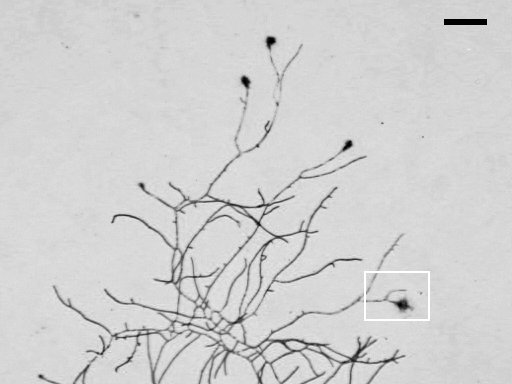
\includegraphics[width=6.5cm]{../C3/BurstTipsLoMag}}}
	\hspace{0.5cm}
	\subfloat[]{\label{fig:BurstTipsb}\fbox{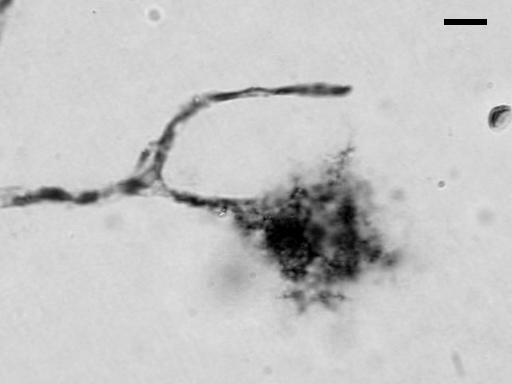
\includegraphics[width=6.5cm]{../C3/BurstTipHiMag}}}
	\caption{Appearance of hyphal tips of \emph{Aspergillus oryzae} when samples are dried without fixative prior to staining. (a) $\times 100$; bar \mic{100}. (b) $\times 1,000$; bar \mic{10}.}
	\label{fig:BurstTips}
\end{figure}

The influence of membrane composition on morphology was investigated and found to be significant (Fig.~\ref{fig:Membranes}). While cellulose acetate membranes successfully confined the growth to two dimensions, the membranes were not sufficiently durable and were found to deform easily during processing. Cellulose nitrate membranes with pore sizes greater than \mic{0.45} were also found to be unsuitable, as considerable three-dimensional growth resulted, which is difficult to image and quantify (Fig.~\ref{fig:MembranesHiMag}). This may suggest that the fungus is capable of penetrating certain membranes, although the mechanism involved is not clear.

\begin{figure}[tb]
	\centering
	\subfloat[]{\label{fig:Membranesa}\fbox{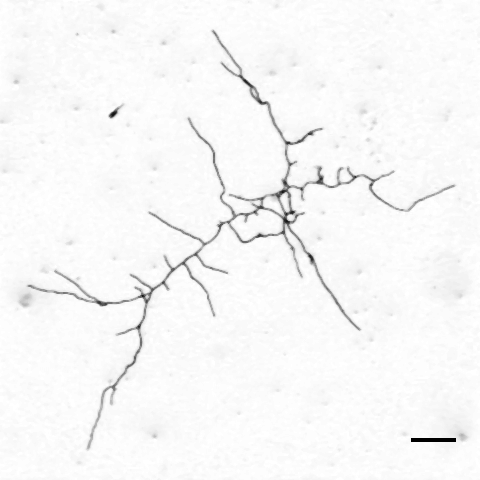
\includegraphics[width=4.5cm]{../C3/Acetate02}}}
	\hspace{0.5cm}
	\subfloat[]{\label{fig:Membranesb}\fbox{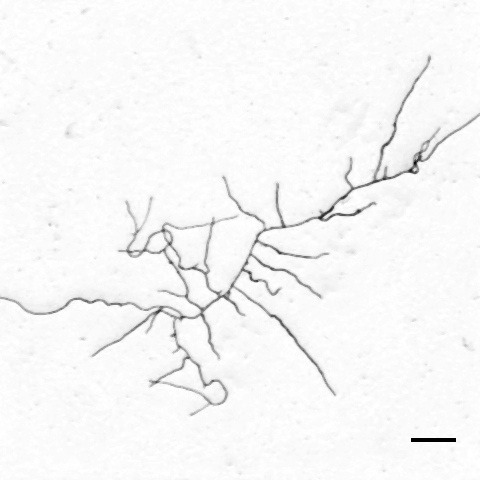
\includegraphics[width=4.5cm]{../C3/Acetate045}}}
	\\
	\subfloat[]{\label{fig:Membranesc}\fbox{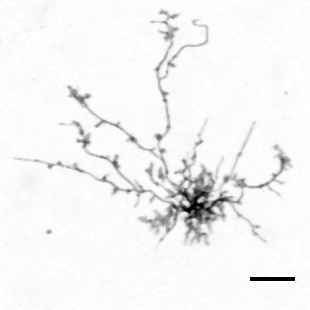
\includegraphics[width=4.5cm]{../C3/Nitrate08}}}
	\hspace{0.5cm}
	\subfloat[]{\label{fig:Membranesd}\fbox{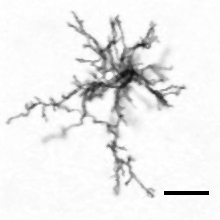
\includegraphics[width=4.5cm]{../C3/Nitrate30}}}
	\caption{Variation in morphological form of \emph{A. oryzae} when grown on different membranes: (a) \mic{0.2} cellulose acetate (Sartorius 11107) (b) \mic{0.45} cellulose acetate (Sartorius 11106) (c) \mic{0.8} cellulose nitrate (Sartorius 11404) (d) \mic{3.0} cellulose nitrate (Sartorius 11302). Bars \mic{100}.}
	\label{fig:Membranes}
\end{figure}

\begin{figure}[htbp]
	\centering
	\subfloat[]{\label{fig:MembranesHiMaga}\fbox{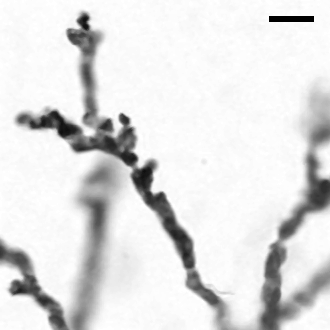
\includegraphics[width=6.5cm]{../C3/Nitrate30HiMag}}}
	\hspace{0.5cm}
	\subfloat[]{\label{fig:MembranesHiMagb}\fbox{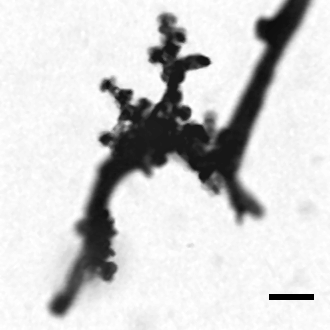
\includegraphics[width=6.5cm]{../C3/MixedEster045HiMag}}}
	\caption{High-magnification images ($\times 1,000$) of \emph{A. oryzae} show extensive three-dimensional growth when cultivated on (a) cellulose nitrate (\mic{3.0} pore size) and (b) mixed cellulose ester membranes (\mic{0.45} pore size). Bars \mic{10}.}
	\label{fig:MembranesHiMag}
\end{figure}

A modification of the assay for the examination of samples taken from submerged culture was also evaluated and found to be suitable for preparations stained with lactophenol cotton blue or calcofluor white (Fig.~\ref{fig:Submerged} \& \ref{fig:CFWHiMag}), a fluorescent stain that has previously been utilised to visualise septation and discriminate between active and non-active hyphal tips in \emph{A. oryzae} \cite{amanullah2002}. The filtration of material and subsequent immobilisation on a membrane reduced the complexity of the conformations from three dimensions to a single focal plane, permitting analysis of the structures present using the routines described in the previous chapter.

\begin{figure}[htbp]
	\centering
	\subfloat[]{\label{fig:Submergeda}\fbox{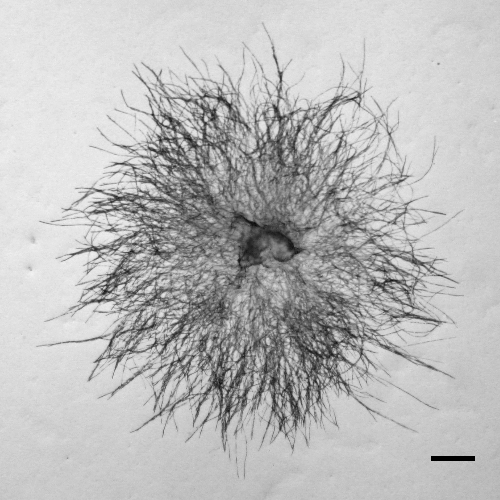
\includegraphics[height=7cm]{../C3/SubmergedSample}}}
	\hspace{0.5cm}
	\subfloat[]{\label{fig:Submergedb}\fbox{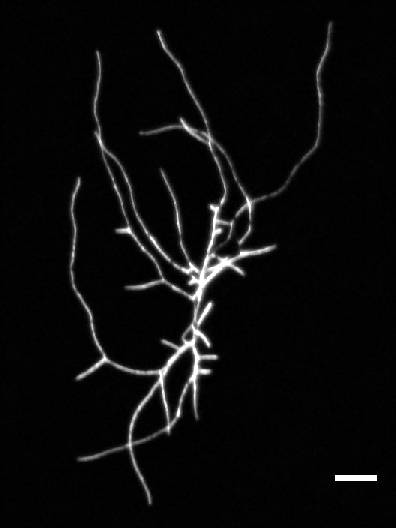
\includegraphics[height=7cm]{../C3/CFWI}}}
	\caption{Samples of \emph{A. oryzae} grown in submerged culture stained with (a) lactophenol cotton blue (bar \mic{50}) and (b) calcofluor white (bar \mic{25}) and immobilised on cellulose nitrate membranes.}
	\label{fig:Submerged}
\end{figure}

\begin{figure}[htbp]
	\centering
	\subfloat[]{\label{fig:CFWHiMaga}\fbox{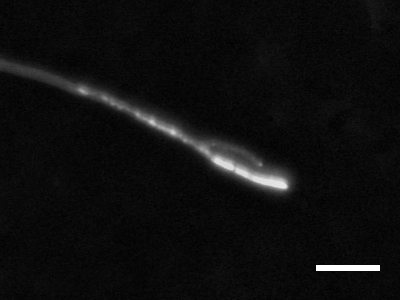
\includegraphics[width=6.5cm]{../C3/CFWActiveTip}}}
	\hspace{0.5cm}
	\subfloat[]{\label{fig:CFWHiMagb}\fbox{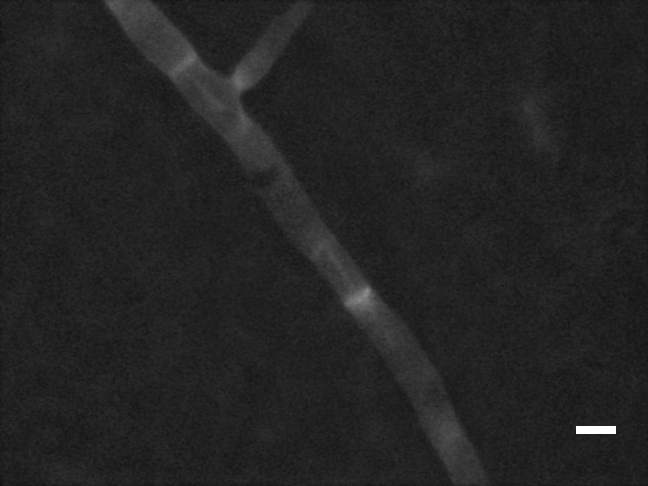
\includegraphics[width=6.5cm]{../C3/CFWSeptation}}}
	\caption{Samples of membrane-immobilised \emph{A. oryzae}, cultivated in submerged medium and stained with calcofluor white, showing (a) \lq active' hyphal region (Bar \mic{20}) and (b) septation (Bar \mic{5}).}
	\label{fig:CFWHiMag}
\end{figure}